\section{Introduction}
\label{sec:introduction}

% GROUP INFORMATION
\hspace{1cm} This project focused on developing a Poker game using the C++11 programming language. It was done in a group of two members, Le Nguyen Anh Tri and Lam Chi Hao (originally three members, but Vo Nhat Tien was unable to contribute due to personal circumstances), for the final project of the course Fundamentals of Programming (CSC10012) at the University of Science, Vietnam National University — Ho Chi Minh City.

\vspace{0.5cm}

\hspace{1cm} Here is our group information for this project:

\begin{table}[ht]
    \centering
    \begin{tabular}{| m{1.75cm} | m{2cm} | m{5cm}| m{2.5cm} |} 
    \hline
    \textbf{} & \textbf{ID} & \textbf{Name} & \textbf{Title} \\ 
    \hline
    1 & 24127034 & Lam Chi Hao & Leader \\ 
    \hline
    2 & 24127567 & Le Nguyen Anh Tri & Member \\ 
    \hline
    \end{tabular}
    \caption{Information of Group 02 member.}
    \label{tab:group-information}
\end{table}

\hspace{1cm} Group management and communication were pretty simple in our two-man team. Messenger served us for fast discussions, while GitHub was used for versioning and collaboration. This simplicity excluded any formal work management board or a developed communication plan. So, roles were divided quite clearly: one team member worked on core game logic, while the second was developing a GUI. Then we will take our time to review the code, test, and make merges towards the end that would bring everything together as needed.

\vspace{0.5cm}

\hspace{1cm} This is our table of contributions for this project, which shows the work we have done.

\begin{table}[ht]
    \centering
    \begin{tabular}{|m{4cm}|m{2cm}|m{2cm}|m{2cm}| m{2cm}|}
    \hline
    \textbf{Problem} & \textbf{Rubric} & \textbf{24127034} & \textbf{24127557} & \textbf{24127567} \\
    \hline
    Standard features & - &  &  &  \\
    \hline
    Initialization & 20 & 5 & 0 & 15 \\
    \hline
    Dealing & 20 & 0 & 0 & 20 \\
    \hline 
    Gameplay & 20 & 0 & 0 & 20 \\
    \hline
    Player's information & 20 & 5 & 0 & 15 \\
    \hline
    Advanced features & - &  &  &  \\
    \hline 
    Draw poker & 30 & 15 & 0 & 15 \\
    \hline
    5-card stud & 30 & 0 & 0 & 0 \\
    \hline
    Color / Sound effects & 30 & 30 & 0 & 0 \\
    \hline
    Leader board & 30 & 10 & 0 & 20 \\
    \hline
    Hash password & 10 & 0 & 0 & 10 \\
    \hline
    Makefile & 10 & 5 & 0 & 5 \\
    \hline
    % Creations & 30 / each & Score & Score & Score \\
    % \hline
    Report & - &  &  &  \\
    \hline
     & 100 & 70 & 0 & 30 \\
    \hline
    & Total & 135 & 0 & 140 \\
    \hline
    \end{tabular}
    \caption{Table of contribution}
    \label{tab:contribution-table}
\end{table}

\hspace{1cm} This project breaks into three significant parts, which are the core game logic, the GUI, and the testing process, which make up the majority of the work. The core game logic was the most challenging part, as it required a deep understanding of the game rules and the ability to implement them in C++. The GUI was the most time-consuming part, as it required a lot of trial and error to get the layout and design right. The testing process was the most tedious part, as it required a lot of manual testing to ensure that the game was bug-free and worked as expected. Each part of the project had its challenges, but we were able to overcome them by working together and supporting each other throughout the process, more details will be discussed in each of the following sections.

\vspace{0.5cm}

\hspace{1cm} To enhance the project a little further, we used the SDL2 library to create a graphical user interface for the Poker game. Such a GUI makes interactions with the game much easier and fun. It gives good visual clarity so that one understands the actual happening of the game better. In that way, by integrating SDL2 into our project, we made it more fun, not to mention challenging, as well.

\subsection{About the Poker Game}
\label{subsec:about-the-poker-game}

\subsubsection{Poker Hand Rakings}
\label{subsubsec:poker-hand-rankings}
\hspace{1cm} In Poker, a hand comprises five cards, regardless of whether the cards are from a single deck or different decks, provided the number is five altogether. Below are the official poker hand rankings, in order from highest to lowest.

\begin{enumerate}
    \item \textbf{Royal Flush}: The best possible poker hand, formed by the Ace, King, Queen, Jack, and 10, all of the same suit, for example, hearts. (Note: This hand is not implemented in our project since it is very rare and not called for in the project specification.)
    \item \textbf{Straight Flush}: Five sequential cards all of one suit (such as 9, 8, 7, 6, 5, all hearts).
    \item \textbf{Four of a Kind}: Four cards of one rank (such as four Aces).
    \item \textbf{Full House}: Three cards of one rank and two cards of another rank (such as three Kings and two 4s).
    \item \textbf{Flush}: Any five cards of the same suit, but not in sequential order (such as 2, 4, 6, 9, King, all in diamonds).
    \item \textbf{Straight}: Five consecutive cards of different suits, like 10 of hearts, Jack of spades, Queen of diamonds, King of clubs, Ace of hearts.
    \item \textbf{Three of a Kind}: Three cards of the same rank, such as three 7s.
    \item \textbf{Two Pair}: Two cards of one rank and two cards of another rank, such as two 5s and two 9s.
    \item \textbf{One Pair}: Two cards of the same rank, such as two 8s.
    \item \textbf{High Card}: If no other hand is made, then the highest card played becomes the rank (such as King, 10, 8, 6, 4; this would be a "King-high" hand).
\end{enumerate}

\hspace{1cm} In all, there are 10 possible poker hands that range from the highest, Royal Flush, to the lowest, High Card. However, in this project, we will implement only hands ranked from Straight Flush to High Card due to the requirements of our project, since it is too rare to happen and the project requirements do not include this as well.

\subsubsection{Poker Game Variants}
\label{subsubsec:poker-game-variants}

\hspace{1cm} Based on that information, there are a lot of variants of Poker, and each has its own rules and way of playing. Some popular variants includes:

\begin{enumerate}
    \item \textbf{Texas Hold'em}: Each player is dealt two private cards, and then five community cards are turned over on the table; players can use any number of these seven cards in attempting to build the highest possible five-card hand.
    \item \textbf{Draw Poker}: Players are dealt five cards and can choose to discard and replace some of them (typically 1 to 3 cards at a time). After this, the player with the best hand wins. The gameplay is structured as follows:
    \begin{itemize}
        \item \textbf{Round 1}: All players are dealt 5 cards each. Players must now decide whether to play by selecting "raise", "call" or "fold".
        \item \textbf{Round 2}: Players can discard and replace one to three cards once (in some versions, if a player has an Ace, he/she can discard four cards and draw four new ones).
        \item \textbf{Round 3}: Players decide again to either "raise", "call", or "fold" depending on their now improved hands.
        \item \textbf{Round 4}: Hands are revealed, and the player with the highest hand wins.
    \end{itemize}
    \item \textbf{Stud Poker}: Some cards are dealt face up and others face down, with several rounds of betting. The highest five-card hand wins the game.
    \item \textbf{Simplified Poker}: This is a Poker variant, included in the project requirements, and is subject to the rules listed below: Each player is initially dealt 5 cards. The player with the highest-ranking hand wins. In case of a tie, when two players hold the same hand, it is won by the player with the highest-ranking card. If two or more players have the same hand and the same high card, then the pot is divided equally.
\end{enumerate}

\hspace{1cm} We are going to implement two game variants: Simplified Poker and Draw Poker. Even though the Simplified Poker game fulfilled all the basic requirements set in the project, we felt it was a bit simple and basic. In order to make the project exciting and challenging, we decided to implement the Draw Poker variant. This is an extension of the framework set by the Simplified Poker game, further allowing us to fulfill some of the advanced requirements stipulated in the project.

\subsection{Class structure of the Poker Game}
\label{subsec:class-structure-of-the-poker-game}

\hspace{1cm} In this project, we have deliberately avoided creating separate, isolated codebases for each game mode that we would like to have. Instead, we designed a unified structure, which contains all game modes under one implementation. This will let us take advantage of the object-oriented features of C++ - that is classes introduced in C++11—to achieve modularity and expandability. By doing so, we can easily modify or extend the project with more game modes in the future without rewriting the whole codebase.


\subsubsection{Class Design}
\label{subsubsec:class-design}

\hspace{1cm} The game of Poker was implemented by using the C++ programming language with SDL2 library and IDE Visual Studio Code. For this, we used the C++11 class feature to design and implement the game. In fact, this usage of classes is beyond the basic requirements of the project. We did it for the following two main reasons:

\begin{enumerate}
    \item \textbf{Pratical Learning}: This exercise used classes, which is good programming practice and prepares us for future, more complex projects.
    \item \textbf{Efficiency}: Classes allow for encapsulation of data and methods, making it easier to extend functionality and organize compared to the traditional struct in C99.
\end{enumerate}

\hspace{1cm} In this project, we used classes in a way similar to how \texttt{struct} would be used in C99, with the added flexibility - thanks to encapsulation - of being able to pack both data and behavior. This allowed us to create better organized code that is maintainable and more readable.

\vspace{0.5cm}

\hspace{1cm} The classes we used in this project are as follows. (About the details, we will explain each of the classes we have implemented for this project in the \hyperref[sec:implementation-of-the-poker-game]{Implementation} section).
\begin{enumerate}
    \item \textbf{\texttt{Card}}: This class represents a single card in the deck. It contains two private members: \texttt{enum Ranks} and \texttt{enum Suits}. The class also contains some public methods for debug purpose that returns the card in the form of a string.
    \item \textbf{\texttt{Deck}}: This class represents a standard 52-card deck. This class has methods for handling things like shuffling, dealing, and resetting the deck.
    \item \textbf{\texttt{Strength}}: This class represents the strength of a hand in Poker based on what we've discussed in the \hyperref[subsubsec:poker-hand-rankings]{Poker Hand Rankings}, which containing methods to evaluate and compare hands.
    \item \textbf{\texttt{Hand}}: This class represents a hand of cards in the game, help us handling things like sorting and evaluating the hand of players.
    \item \textbf{\texttt{Storage}}: Represent a storage that stores player information, handling reading and writing player data to a file.
    \item \textbf{\texttt{Leaderboard}}: Represents the leaderboard, handling reading and writing leaderboard data to a file.
    \item \textbf{\texttt{Player}}: Contains all necessary player information used in the game. This class encapsulate various attributes associated with the players. It includes public memeber variables such as \texttt{string username}, \texttt{float chips}, \texttt{unsigned int winningStrategy[9]} (since there are 9 combinations of Poker hand being covered in this project), and so on.
    \item \textbf{\texttt{Gameplay}}: This class encapsulates the core components such as the deck of cards via \texttt{Deck} and player data via \texttt{Player}. It provides methods to initialize the game with players and bots, deal cards, manage player actions, determine the winner, and maintain a leaderboard. By centralizing these functionalities, the \texttt{Gameplay} class ensures that the game logic is organized, making the codebase easier to maintain and extend. This class is essential for coordinating the various elements of the game, ensuring a smooth and coherent gameplay experience.
    \item \textbf{\texttt{Lobby}}: This class manages the players and bots waiting for a game to start. It provides methods to add and remove players via username and handle the number of players in the lobby. By keeping track of the players and bots in the lobby, the \texttt{Lobby} class ensures that the game can start with the correct number of players.
    \item \textbf{\texttt{GameEngine}}: This is the core component of the entire game application, responsible for managing the main game loop and handling the game states and events. It manages things related to initialization, event handling, updating, rendering, and the cleanup processes. This class ensure the game run correctly, make things easier to scale up and maintain.
\end{enumerate}

\subsubsection{Class Diagram}
\label{subsubsec:class-diagram}
\hspace{1cm} The following diagram illustrates the main classes and their relationships in the poker game:

\begin{figure}[H]
    \centering
    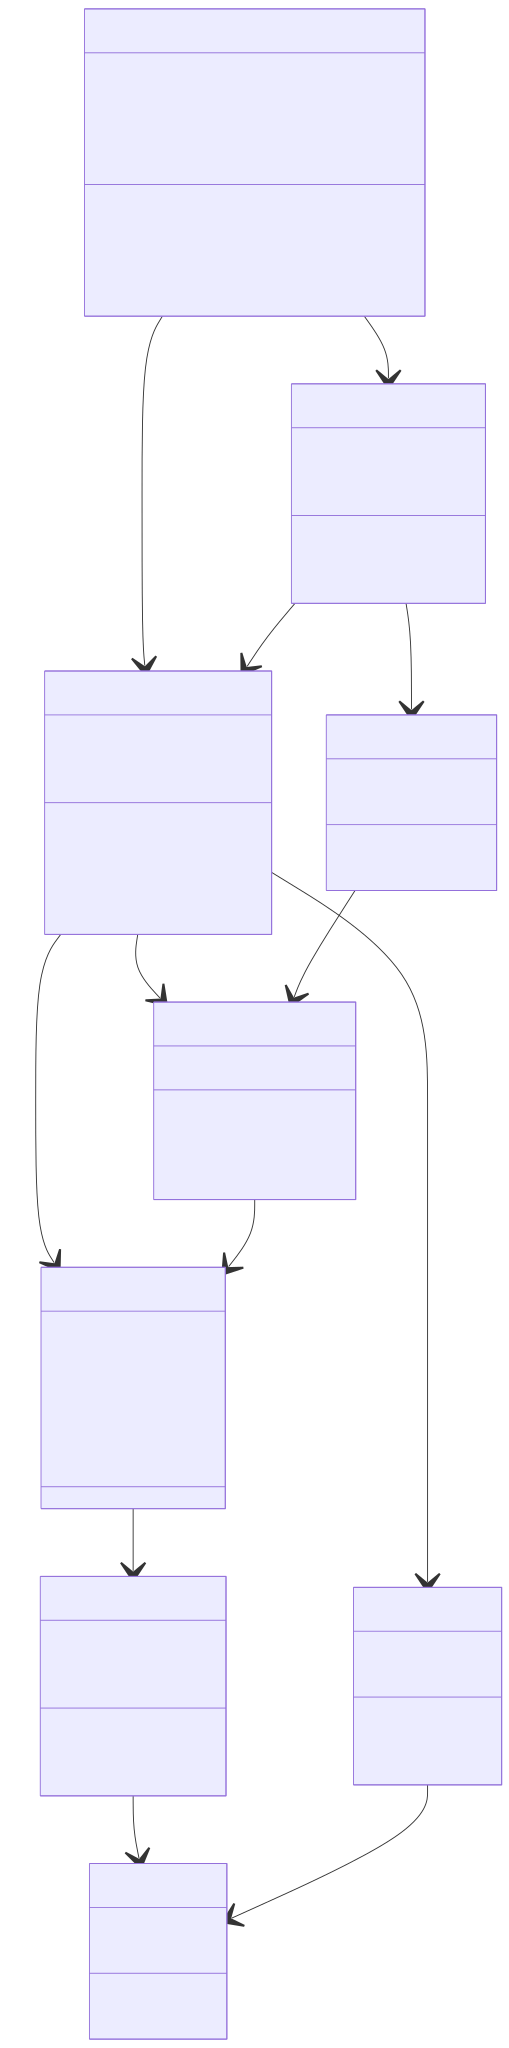
\includegraphics[width=125pt]{figures/class-diagram.png}
    \caption{Class Diagram of the Poker Game}
    \label{fig:class-diagram}
\end{figure}

\subsection{Naming Convention of the Project}
\label{subsec:naming-convention-of the-project}

\hspace{1cm} For this part of the report, we will discuss the project structure, including the folder structure, file structure, variable, constant, class, as well as struct naming conventions.

\vspace{0.5cm}

\hspace{1cm} The naming convention is a set of rules for choosing the character sequence to represent the name of a variable, constant, function, class, file, folder, or other entity in the source code. The naming convention is essential because it helps the reader understand the code more easily and quickly. In this project, we follow the naming convention below:

\subsubsection{Folder}
\label{subsubsec:folder}

\hspace{1cm} We decide that all folder names are named in lowercase and separated by an underscore. There are two main rules for naming folders in our project:

\begin{itemize}
    \item \textbf{lowercase}: All characters in the folder name are lowercase.
    \item \textbf{Underscore}: If the folder name consists of multiple words, separate them with an underscore.
\end{itemize}

\subsubsection{File}
\label{subsubsec:file}

\hspace{1cm} We decide that all file names are named in lowercase and separated by an underscore or hyphen. There are three main rules for naming files in our project:

\begin{itemize}
    \item \textbf{lowercase}: Only one exception is our main file, which is named \textbf{main.cpp}.
    \item \textbf{CamelCase}: We decide that all of the header files and source files are named in CamelCase.
    \item \textbf{Underscore \& hyphen}: This is for files in SDL2 libraries, which are named in lowercase and separated by an underscore. Besides that, our files in assets are named in lowercase and separated by an underscore or hyphen.
\end{itemize}

\subsubsection{Variable, constant, class, struct}
\label{subsubsec:variable-constant-class-struct}

\hspace{1cm} We decide that all of the variables, constants, classes, and structures are named in camelCase, CamelCase, and ALL\_CAPS. There are three main rules for naming variables, constants, classes, and structures in our project:

\begin{itemize}
    \item \textbf{camelCase}: We decide that all of the variables are named in camelCase. Notice that the first letter of the first word is lowercase, and the first letter of the following words is uppercase.
    \item \textbf{CamelCase}: For classes and structures in our project, we decide that all of the classes and structures are named in CamelCase. Notice that the first letter of each word is uppercase.
    \item \textbf{ALL\_CAPS}: We decide that all of the constants are named in ALL CAPS. Notice that if the constant consists of multiple words, we will separate them with an underscore.
\end{itemize}

\subsubsection{Function Prototype and Definition}
\label{subsubsec:function-prototype-definition}

\hspace{1cm} We decide that all of the functions are named in camelCase. Notice that the first letter of the first word is lowercase, and the first letter of the following words is uppercase.

\subsection{Folder structure of the Project}
\label{subsec:folder-structure-of-the-project}

\hspace{1cm} After discussing, we decided that the project structure will be organized as follows. This structure ensures that the project is well-organized, making it easier to navigate, maintain, and scale. Each folder and file has a specific purpose, and the naming conventions are designed to be intuitive and consistent. Below is a detailed breakdown of the project structure:

\begin{itemize}
    \item \textbf{src}: Contains all source code files written in C++. There are two subfolders with two main categories of source code files.
    \begin{itemize}
        \item \textbf{core}: Contains all the source files related to the core mechanics of the game.
        \item \textbf{gui}: Contains all the source files related to the graphical user interface of the game.
    \end{itemize}
    \item \textbf{include}: Contains all header files. There are two subfolders with two main categories of header files.
    \begin{itemize}
        \item \textbf{core}: Contains all the header files related to the core mechanics of the game.
        \item \textbf{gui}: Contains all the header files related to the graphical user interface of the game.
    \end{itemize}
    \item \textbf{bin}: Contains all executable files, object files, and dynamic libraries. There is a subfolder called obj. Inside the obj folder, there are two subfolders with two main categories of object files.
    \begin{itemize}
        \item \textbf{core}: Contains all the object files related to the core mechanics of the game.
        \item \textbf{gui}: Contains all the object files related to the graphical user interface of the game.
    \end{itemize}
    \item \textbf{assets}: Contains all assets used in the project. There are three subfolders inside our assets folder.
    \begin{itemize}
        \item \textbf{imgs}: Contains all images used in the project. There are images for backgrounds, buttons, cards, cursor, and icons for our game application.
        \item \textbf{audios}: Contains all sounds used in the project. There are audios for background music, button click sound, card shuffle sound, and card flip sound.
        \item \textbf{fonts}: Contains all fonts used in the project. There are fonts for the game title, game buttons, and game text.
    \end{itemize}
    \item \textbf{libs}: Contains all libraries used in the project.
    \begin{itemize}
        \item \textbf{SDL2}: Contains all SDL2 libraries. This is our main library for creating the graphical user interface.
        \item \textbf{cmake}: Contains all CMake libraries.
    \end{itemize}
    \item \textbf{report}: Contains all report files which are source code files written in LaTeX.
    \begin{itemize}
        \item \textbf{contents}: Contains all the contents of the report. We want to keep the report organized, so we separate the report into multiple files and put them in the contents folder.
        \item \textbf{figures}: Contains all figures used in the report. The figures are images, graphs, tables, etc.
    \end{itemize}
\end{itemize}

% ------------------- THE END ------------------- %